% !TEX program=lualatex
\RequirePackage{luatex85}
\documentclass[11pt,tikz]{standalone}

\usepackage{luatextra} % also loads fixltx2e, fontspec, xunicode
\usepackage{microtype} % Slightly tweak font spacing for aesthetics
\usepackage{mathtools}
\usepackage{amsmath}
\usepackage{unicode-math}
\usepackage{xcolor}

\usepackage{tikz}
\usetikzlibrary{shapes,arrows,positioning,matrix}

\setmainfont{TeX Gyre Heros}
\setmathfont{Latin Modern Math}
\setmonofont{Source Code Pro}

\definecolor{colorR}{RGB}{228,26,28}    % RED
\definecolor{colorB}{RGB}{55,126,184}   % BLUE
\definecolor{colorG}{RGB}{77,175,74}    % GREEN
\definecolor{colorP}{RGB}{152,78,163}   % PURPLE
\definecolor{colorO}{RGB}{255,127,0}    % ORANGE
\definecolor{colorY}{RGB}{255,255,51}   % YELLOW
\definecolor{colorBn}{RGB}{166,86,40}   % BROWN
\definecolor{colorPk}{RGB}{247,129,191} % PINK
\definecolor{colorGy}{RGB}{153,153,153} % GRAY
\definecolor{asublue}{RGB}{0,163,224}

\tikzstyle{aln}=[matrix of nodes]
\tikzstyle{best}=[fill=asublue!25]
\tikzstyle{lab}=[font=\normalsize]

\newcommand{\e}[1]{\textcolor{colorR}{#1}}

\begin{document}
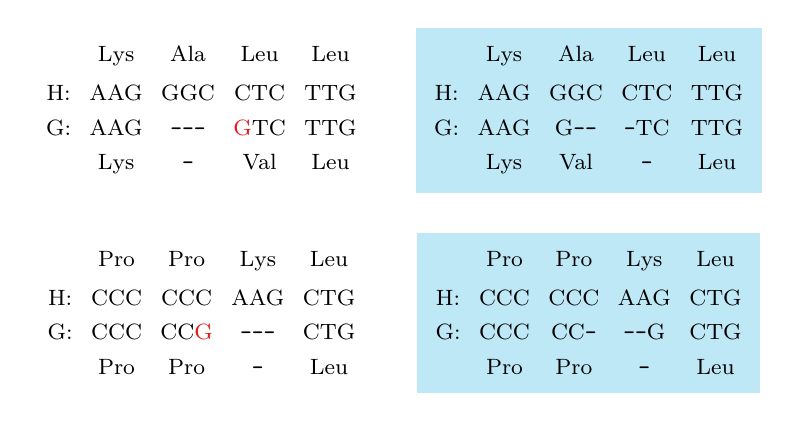
\begin{tikzpicture}[node distance=5mm,font=\footnotesize]

%%%%%
% ENSG00000131203.fasta

% prank
\matrix (a)[aln] {
   & Lys & Ala & Leu & Leu \\
H: & AAG & GGC & CTC & TTG \\
G: & AAG & \verb|---| & \e{G}TC & TTG \\
   & Lys & \verb|-| & Val & Leu \\
};

% improved version
\matrix (b)[aln,right=of a,best] {
   & Lys & Ala & Leu & Leu \\
H: & AAG & GGC & CTC & TTG \\
G: & AAG & G\verb|--| & \verb|-|TC & TTG \\
   & Lys & Val & \verb|-| & Leu \\
};

%%%%%
%ENST00000296238.4

% prank
\matrix (c)[aln,below=of a] {
   & Pro & Pro & Lys & Leu \\
H: & CCC & CCC & AAG & CTG \\
G: & CCC & CC\e{G} & \verb|---| & CTG \\
   & Pro & Pro & \verb|-| & Leu \\
};

% improved version
\matrix (d)[aln,below=of b,best] {
   & Pro & Pro & Lys & Leu \\
H: & CCC & CCC & AAG & CTG \\
G: & CCC & CC\verb|-| & \verb|--|G & CTG \\
   & Pro & Pro & \verb|-| & Leu \\
};

%%%%%

% \draw (a.north west) node[lab,anchor=center] (dlab) {\textbf{a)}};
% \draw (dlab |- c.north west) node[lab,anchor=center] {\textbf{b)}};

\node[] () [below = 0.2em] at (d.south) {};

\end{tikzpicture}
\end{document}
